% Figure 4: (a) equivalent compute of frontier-model knowledge; (b) paired KB-injection lifts
% Model identities anonymized (Frontier-1 strongest ... Frontier-10 weakest, by closed-book accuracy).
\documentclass[tikz,border=8pt]{standalone}
% Shared preamble for SAI taxonomy standalone figures.
% Self-contained: no MetaCircle dependency; colors match the paper palette.
\usepackage{amsmath,amssymb}
\usetikzlibrary{arrows.meta}
\definecolor{MetaPurple}{HTML}{6D3BD1}
\definecolor{MetaViolet}{HTML}{9B5DE5}
\definecolor{MetaCoral}{HTML}{D76A7A}
\definecolor{MetaInk}{HTML}{16131D}
\definecolor{MetaGray}{HTML}{F4F2F7}
\definecolor{MetaMidGray}{HTML}{6E6875}
\newcommand{\Lk}{\mathcal{L}_1}
\newcommand{\Ll}{\mathcal{L}_2}
\newcommand{\Ls}{\mathcal{L}_3}
\newcommand{\Op}[1]{\textsc{#1}}
\newcommand{\universe}{\Omega}
\newcommand{\kb}{\mathcal{K}}
\newcommand{\cell}{\omega}

\begin{document}
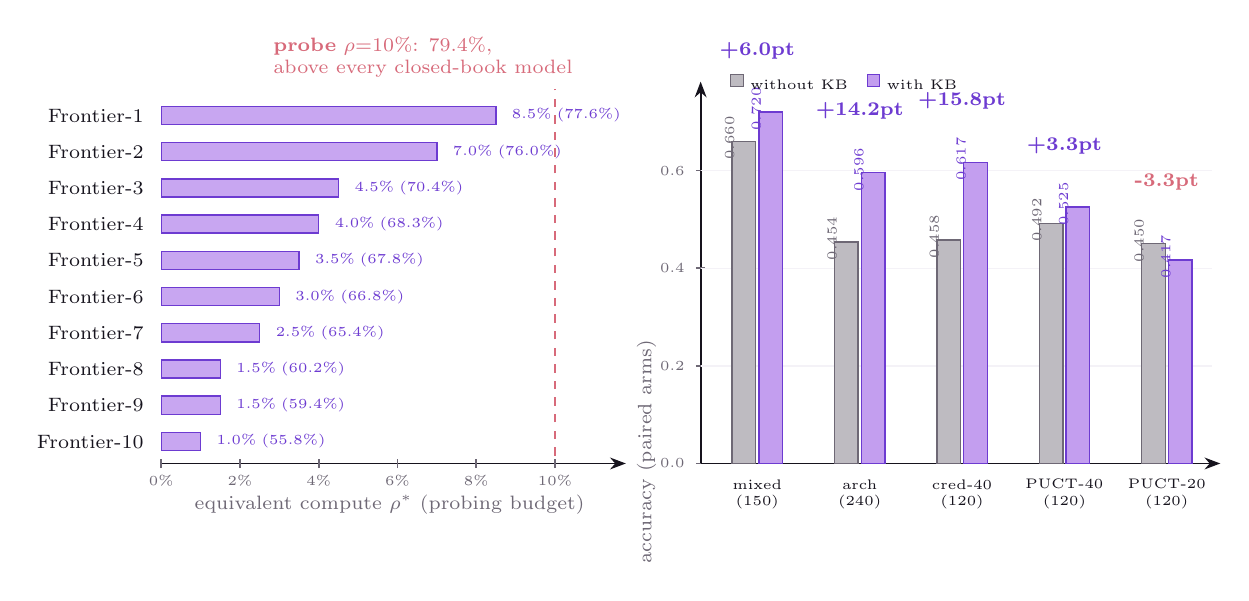
\begin{tikzpicture}[font=\small]
% ============ left panel: equivalent compute ============
\begin{scope}
  \draw[-{Stealth[length=2mm]}, line width=0.7pt, MetaInk] (3.0,0.2) -- (8.9,0.2);
  \foreach \v in {0,2,4,6,8,10} {
    \draw[line width=0.6pt, MetaMidGray] ({3.0+\v*0.5},0.14) -- ({3.0+\v*0.5},0.26);
    \node[font=\tiny, text=MetaMidGray] at ({3.0+\v*0.5},-0.02) {\v\%};
  }
  \node[font=\scriptsize, text=MetaMidGray] at (5.9,-0.32) {equivalent compute $\rho^*$ (probing budget)};
  \foreach \model/\rho/\acc [count=\n from 0] in {%
    Frontier-1/8.5/77.6,%
    Frontier-2/7.0/76.0,%
    Frontier-3/4.5/70.4,%
    Frontier-4/4.0/68.3,%
    Frontier-5/3.5/67.8,%
    Frontier-6/3.0/66.8,%
    Frontier-7/2.5/65.4,%
    Frontier-8/1.5/60.2,%
    Frontier-9/1.5/59.4,%
    Frontier-10/1.0/55.8} {
    \pgfmathsetmacro{\yy}{4.62-\n*0.46}
    \node[font=\scriptsize, anchor=east, text=MetaInk] at (2.9,\yy) {\model};
    \fill[MetaViolet!55] (3.0,{\yy-0.115}) rectangle ({3.0+\rho*0.5},{\yy+0.115});
    \draw[MetaPurple, line width=0.5pt] (3.0,{\yy-0.115}) rectangle ({3.0+\rho*0.5},{\yy+0.115});
    \node[font=\tiny, anchor=west, text=MetaPurple] at ({3.08+\rho*0.5},\yy) {\rho\%\;(\acc\%)};
  }
  \draw[MetaCoral, line width=1.0pt, dashed] (8.0,0.3) -- (8.0,4.95);
  \node[font=\scriptsize, text=MetaCoral, align=left, anchor=south west] at (4.3,4.98) {\textbf{probe} $\rho{=}10\%$: 79.4\%,\\ above every closed-book model};
\end{scope}
% ============ right panel: paired KB lifts ============
\begin{scope}[shift={(9.35,0)}]
  \draw[-{Stealth[length=2mm]}, line width=0.7pt, MetaInk] (0.5,0.2) -- (0.5,5.05);
  \foreach \v in {0.0,0.2,0.4,0.6} {
    \pgfmathsetmacro{\yy}{0.2+\v*6.2}
    \draw[line width=0.6pt, MetaMidGray] (0.44,\yy) -- (0.56,\yy);
    \node[font=\tiny, text=MetaMidGray, anchor=east] at (0.42,\yy) {\v};
    \draw[MetaGray, line width=0.5pt] (0.5,\yy) -- (7.0,\yy);
  }
  \node[rotate=90, font=\scriptsize, text=MetaMidGray, anchor=south] at (0.06,0.35) {accuracy (paired arms)};
  \draw[-{Stealth[length=2mm]}, line width=0.7pt, MetaInk] (0.5,0.2) -- (7.1,0.2);
  \foreach \glabel/\wo/\wi/\lift [count=\j from 0] in {%
    {mixed\\(150)}/0.660/0.720/+6.0,%
    {arch\\(240)}/0.454/0.596/+14.2,%
    {cred-40\\(120)}/0.458/0.617/+15.8,%
    {PUCT-40\\(120)}/0.492/0.525/+3.3,%
    {PUCT-20\\(120)}/0.450/0.417/-3.3} {
    \pgfmathsetmacro{\xg}{0.90+\j*1.30}
    \pgfmathsetmacro{\hwo}{0.2+\wo*6.2}
    \pgfmathsetmacro{\hwi}{0.2+\wi*6.2}
    \pgfmathsetmacro{\hl}{0.2+max(\wo,\wi)*6.2+0.78}
    \fill[MetaMidGray!45] (\xg,0.2) rectangle ({\xg+0.30},\hwo);
    \draw[MetaMidGray, line width=0.5pt] (\xg,0.2) rectangle ({\xg+0.30},\hwo);
    \node[font=\tiny, text=MetaMidGray, rotate=90, anchor=south] at ({\xg+0.15},{\hwo+0.04}) {\wo};
    \fill[MetaViolet!60] ({\xg+0.34},0.2) rectangle ({\xg+0.64},\hwi);
    \draw[MetaPurple, line width=0.5pt] ({\xg+0.34},0.2) rectangle ({\xg+0.64},\hwi);
    \node[font=\tiny, text=MetaPurple, rotate=90, anchor=south] at ({\xg+0.49},{\hwi+0.04}) {\wi};
    \pgfmathparse{ifthenelse(\lift<0,"MetaCoral","MetaPurple")}
    \edef\liftcol{\pgfmathresult}
    \node[font=\scriptsize\bfseries, text=\liftcol] at ({\xg+0.32},\hl) {\lift pt};
    \node[font=\tiny, text=MetaInk, align=center, anchor=north] at ({\xg+0.32},0.12) {\glabel};
  }
  \node[font=\tiny, align=left, text=MetaInk, anchor=west] at (0.75,5.05) {%
    \tikz[baseline=-1pt]{\fill[MetaMidGray!45] (0,0) rectangle (0.16,0.16);\draw[MetaMidGray,line width=0.4pt] (0,0) rectangle (0.16,0.16);} without KB\quad
    \tikz[baseline=-1pt]{\fill[MetaViolet!60] (0,0) rectangle (0.16,0.16);\draw[MetaPurple,line width=0.4pt] (0,0) rectangle (0.16,0.16);} with KB};
\end{scope}
\end{tikzpicture}
\end{document}
